\chapter{Changes to Design} \label{design-changes}

While implementing the design we envisioned in our design phase, we decided do modify it in some ways.
Our decisions were based on the knowledge we gained in this phase.

As most changes affect both the \gls{backend} and the \gls{frontend}, we decided to keep them as one list.
They are ordered by size, with the largest modifications listed first.
Some minor changes to implementation details, like "design document did not mention constructor" where the constructor adds 2 lines of code, are omitted to improve readability.

\section{Support for multiple KinematicUnits}

In the design phase, we assumed that there would only be one KinematicUnit in each \gls{ice} network.
However, we have since learned that there can be an arbitrary amount of KinematicUnits.
This required changing both the API specification and the service implementation:

The KinematicUnit is now able to provide data for all KinematicUnits. 
Additionally, it exposes a new endpoint that provides a list of known KinematicUnits to clients of the API.

\begin{figure}[h!]
    \centering
    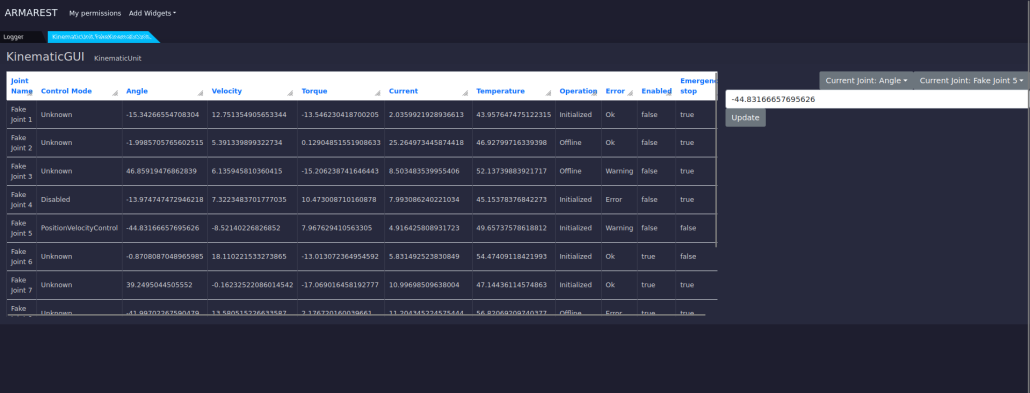
\includegraphics[width=0.8\linewidth]{images/kinematic.png}
\end{figure}

\section{Service for checking tokens}

We originally designed our API to not have an explicit endpoint to check authentication tokens.
This kept the API simple, but we have now decided that improving the user experience is more important:\\
All API clients (currently, the \gls{frontend}) should have a simply way to verify that the token provided to them is valid.

Therefore, we created a new service: check\_token.\\
It only contains one HTTP endpoint: GET /api/v1/check\_token, which is secured (requires authentication) and returns a 204 No Content response.
Therefore, if the request is authenticated, it receives a simple 204 response. If it is not authenticated, 
the \gls{backend} responds with either an error 401 Unauthorized or 403 Forbidden, just like all other endpoints in our other services behave.

The \gls{frontend} accesses this endpoint when a user enters an autentication token in the login page.
It gives feedback to the end user based on the response it received.

\begin{figure}[h!]
    \centering
    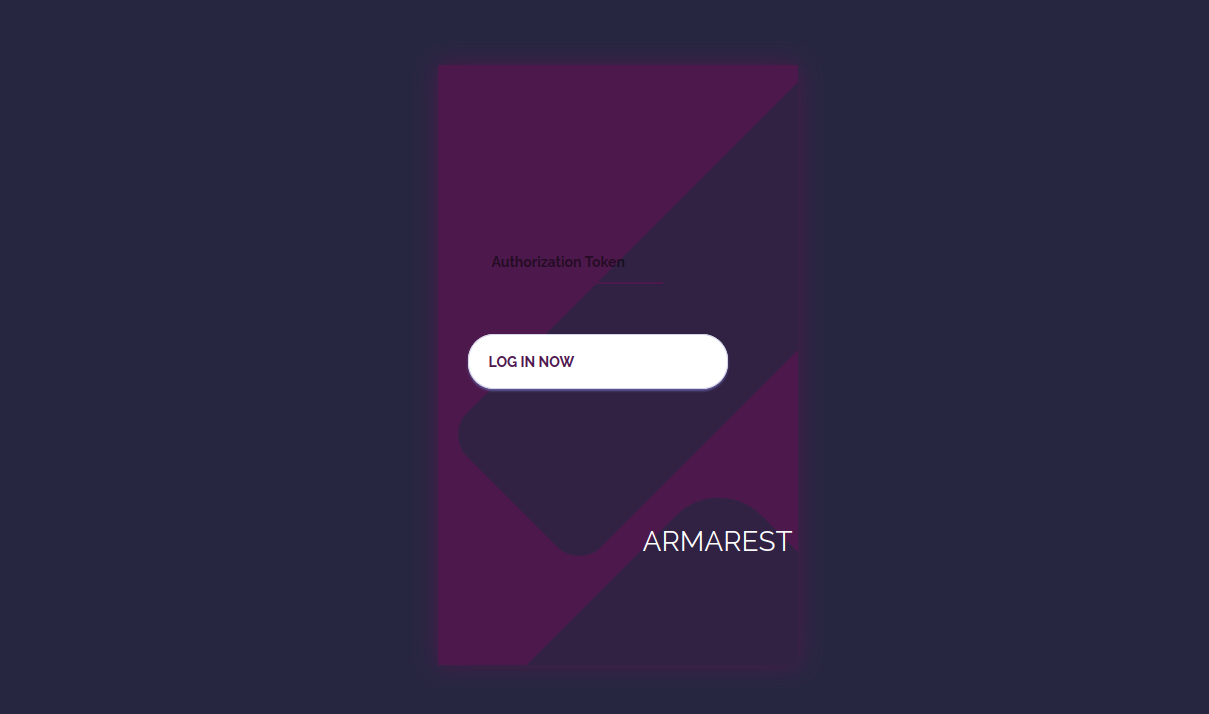
\includegraphics[width=0.8\linewidth]{images/login.png}
\end{figure}

\section{Dependencies}

We planned on using the `GoldenLayout' library in our \gls{frontend} to allow the end user to resize and move widgets in the workspace.
However, we found a different library that better fits our needs: ProjectStorm's `React Workspaces'.
It provides us with the same functionality as GoldenLayout, but had better integration into React.

To be more specific, GoldenLayout expected to be above all react components in our hierarchy.
However, this would mean placing the navbar, login page etc. into the GoldenLayout, or to create them without React.
Neither of these options were appealing to us, therefore, we chose to use a different library for the same purpose.

The \gls{frontend} now also uses some styling and formatting libraries and utilities, such as Bootstrap and react-table-util.

The \gls{backend} uses the following new dependencies:
\begin{itemize}
    \item typeguard checks the types of all function arguments and return types. By default, it also checks functions in libraries that we use. However, slice2py generates file that are incompatible with type-checking. Therefore, we decided to limit type-checking to our own project and disable checking of our libraries.
    \item pydantic provides us with type-checked data classes that can be serialized to json. The type-checking provided by pydantic is enabled globally and protects our dataclasses everywhere.
    \item pytest is used for our existing unit tests and will be used in the next phase for more tests
    \item flask-cors and pyjwt are small utilities we use to simplify securing our project.
\end{itemize}

\section{Launchers}

The ARMAREST \gls{backend} is now launched through one of two launchers.
Our launchers are responsible for parsing command-line arguments (currently: --no-auth) and initializing the main class.

The default \gls{backend} launcher instantiates a new Armarest object and registers the services in it.
It then calls the run method on the Armarest class to start the \gls{backend} as usual.

The testing server \gls{backend} launcher was created to allow developers of API clients, such as our \gls{frontend}, to use the API with mock data.
This allows for testing even on devices without a connection to the \gls{ice} network of an \gls{armar} robot or simulation.
The data is therefore not provided by \gls{ice}, but is instead procedually created while the testing server is running.
As we only swap out the data source, most of the \gls{backend} classes are used in the testing server as well.
This demonstrates that our split between business logic in our service cores and the \gls{ice} package is working as intended.

\section{Main Page class}

We added a MainPage class to the \gls{frontend} that is responsible for rendering either the LoginPage or the Workspace.
It also fetches some initial data, such as which KinematicUnits and which remote gui tabs are known to the \gls{backend}.

\section{Widget class}

In the initial design, the widget class was designed as the common parent class of all widgets in the frontend. However, we have decided to change the design to a new approach: 

The widget class now stores the component type that can render the widget and the props that it should receive. This allows us to store all widgets even when they are not in the workspace, as they are only instantiated when they are added to the workspace based on the props and type stored in the Widget class.

\section{API changes}

To simplify the implementation in \gls{backend} and \gls{frontend}, the log messages sent by the logger now contain the verbosity as an integer index into an array instead of a string and the timestamp in the \gls{iso8601} format instead of Unix milliseconds.

To reduce the amount of data sent, the RemoteGui /tabs/ endpoint now sends just an array of tab names instead of all tabs with their values. This allows clients to be more specific in which data they actually need, instead of just receiving everything.
